%!TEX root = ../dissertation.tex

\chapter{BlendMe! - The User Study}
\label{chapter:design}
%
This chapter of the document concerns the design and implementation decisions fulfilled when developing the
supporting platform of our user color study. For the sake of simplification when describing and talking about
this platform, we have called it \emph{BlendMe!}, since its purpose is to support the collecting and analysis
of data from color blendings! \par
%
We are going to state the objectives for this user study, concrectly defining the questions which we want to
have answers in the end of the study; then, we will discuss how the \emph{BlendMe!} was implemented, justifying
the decisions taken in each phase of the study. To end this section, we will define some evaluation criteria which
is going to be important for the data cleaning and processing phase of the research.
%
\section{Objectives}
\label{sec:impl_objectives}
%
As seen before, there is a myriad of questions about the usage of color blendings when conveying information,
which remained unanswered. However, only a set of questions is answered in our research, since it is not possible
to reach answers to all questions. Therefore, the goals which we have picked for this User Study are as follows:
%
\begin{enumerate}
	\item Study a way to present color which does not influence color perception.
  \item Understand if there is any psychological organization of color, when detailing color mixtures' components.
  \item If possible, obtain results to ascertain the cultural influence in color perception.
  \item Study the influence of discrete and continuous color scales.
\end{enumerate}
%
Additionally, it is relevant to understand which color model stands as the best to mix colors which are, from a
perceptual point of view, more similar to the users expectation. We have planned to develop this study in two
different strands: in a \textbf{Laboratory Environment}, which will allow us to calibrate and perfectly control the
entire study conditions, and in an \textbf{Online Environment}, which will allow us to disseminate our study to a
larger set of users, even without controlling the calibration of the testing environment). \par
%
The questions which we think define our research goals, for this study, are:
%
\begin{itemize}
	\item \textbf{Q1:} Which Color Model meets best the users' expectations, when blending two colors?
	\item \textbf{Q2:} Is there evidence of a spatial arrangement of colors, when users are indicating possible color
	mixtures' results?
	\item \textbf{Q3:} Are there evidences from differences across demographic groups, such as the age or gender?
\end{itemize}
%
Along the result analysis, each question will meet its answers. These questions will be explored in multiple
threads, such as:
%
\begin{enumerate*}
		\item \textbf{Analyzing the distances of each answer pair to the ideal answers of each color model}, verifying
		which color models had the best and the worst values yielded by the descriptive statistic analysis,
		\item \textbf{Evaluate the results from blendings when the basis is given to the user, against when the result
		of the blending is given},
		\item \textbf{Verify if the color models which have the best and worst results are subtractive or addictive},
		\item \textbf{Analyze the ease of blending colors}, or if
		\item \textbf{There is substantially different results among genders, or different age groups}.
\end{enumerate*}
\\ \\
%
To meet these study requirements, we drafted our study into three different phases: a \textbf{User Profiling Phase},
a \textbf{Calibration Phase}, a \textbf{Color Deficiency Test Phase} and finally, the \textbf{Core Phase}. In the
following section, we detail each of these study phases. \par
%
\section{Designing the \emph{BlendMe!}}
\label{sec:impl_designingsolution}
%
Since we aim to \emph{study to what extent can color blending techniques be used to efficiently and effectively
convey information}, it is important learn from previous results, testing out not only the validity of them but also
some missed opportunities. \par
%
One of the points discussed in section \ref{sec:background_discussion} was the amount of users who performed the study
of Gama and Gonçalves \cite{Gama20141,Gama20142}: it was large enough for their questions. However, considering the
results we aim to achieve with this study, a considerably larger sample of users is the ideal: besides conducting
the study in a laboratory environment, it is mandatory to expand the sample size by performing user studies with
online users, trying to take advantage of the cultural diversity that may arise. \par
%
Therefore, we intended to develop a user study which could support the laboratory controlled environment, while at
the same time supporting the collection of metrics and data from the online users: this is an important consideration,
since the workload when analyzing the results would be dramatically reduced because the data is condensed and gathered
in the same fashion. As referred, the user study was divided onto four different stages: the \textbf{user profiling},
\textbf{calibration testing}, \textbf{color deficiency testing} and, finally, the \textbf{principal part of the study}
where the core information was collected from the users. Each of these phases will be adressed later in this section. \par
%
When brainstorming the ideas for this study, we started with the intention of testing both the blending of two colors and
three colors; we decided that the colors which would be blended were Red (\textbf{R}), Green (\textbf{G}),
Blue (\textbf{B}), Cyan (\textbf{C}), Magenta (\textbf{M}) and Yellow (\textbf{Y}), since they represent each primitive
of the most commonly known Color Models, \ul{RGB (Additive Color Model)} and \ul{CMYK (Subtractive Color Model)}. \par
%
The color models we intended to study: the color models were \textbf{HSV, RGB, CMYK, CIE-L*a*b*} and \textbf{CIE-L*C*h*}.
These color models were picked according to previous studies conducted by Gama and Gonçalves, which have concluded that HSV
and CIE-L*C*h* were the models which generated better results \cite{Gama20141,Gama20142}; the RGB and CMYK were obvious
additions, since they are represented by their primitives and we wanted to compare the users' expectations with two
representative different color model types (additive and subtractive). Lastly, the inclusion of CIE-L*a*b* was due to the fact
that it is the color model which represents the entire range of human perceivable colors. \par
%
Then, we produced a wide spreadsheet of possible blendings of these colors, according to these color models, \textbf{mixed in
pairs of two colors} and \textbf{triples of three colors, without opposed colors in HSV angle}: this generated the total amount
of 183 Color Blendings, being 78 from blendings of two colors and 105 from blendings of three colors. \textbf{There are 15
possible mixtures of two colors}, when combining the previous defined colors: R-G, R-B, G-B, R-C, R-M, R-Y, C-M, M-Y, G-C, G-M,
G-Y, B-C, B-M, B-Y and C-Y; on the other hand, there are 21 possible color mixtures of three colors without opposed colors in the
HSV hue circle: R-G-B, R-B-G, B-G-R, R-M-B, R-B-M, B-M-R, C-G-B, C-B-G, B-G-C, C-M-Y, C-Y-M, Y-M-C, C-M-B, C-B-M, B-M-C, C-G-Y,
C-Y-G, Y-G-C, R-M-Y, R-Y-M and Y-M-R. Figure \ref{fig:table_blends} shows an excerpt of the table produced: depicts the results,
for each color pair, blended according to the five color models chosen.
%
\begin{figure}[htbp]
	\centering
  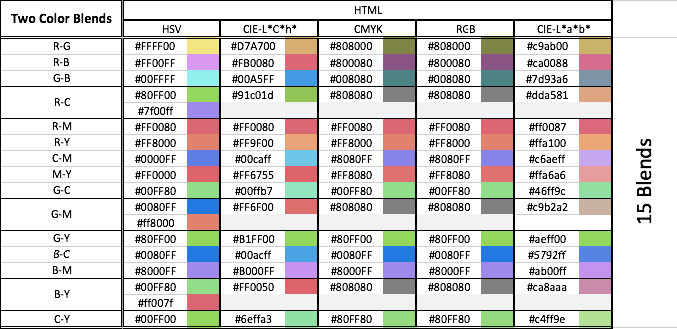
\includegraphics[width=0.8\textwidth]{images/implementation/table_blends.png}
  \caption[Excerpt of Table containg the pre-calculated Color Blends.]{Excerpt of Table containg the pre-calculated Color Blends.}
  \label{fig:table_blends}
\end{figure} \par
%
For the sake of simplicity, we have decided to drop the idea of testing the blendings of three colors, since the blendings of two
colors already produce a generous amount of possible questions. This table was converted to \gls{CSV} file, which will be useful
in the \ul{Core Phase of the study}, which will be explained later. \par
%
This user study was entirely developed used web-development libraries (\emph{e.g.} Bootstrap), technologies (\emph{e.g.} HTML5, Javascript
and CSS) and relational databases (PostgreSQL): these concepts will be adressed in respective sections.
%
\subsection{User Profiling Phase}
\label{subsec:design_profiling}
%
In the \textbf{Profiling Phase}, questions were asked about the Age, Gender, Academic Degree, Nationality and Country of Residence: these
questions helped us conceiving user profiles with key indicators about cultural background and gender relation to results of each test. \par
%
We have drafted ... \par
%
When this phase is concluded, the user will be guided to another stage of the study, to perform the \textbf{Calibration Phase}, where he will be asked to analyze a set of images and answer a pair of questions. \par
%
\subsection{Testing Calibration Phase}
\label{subsec:design_calibration}
%
Performing online tests - specially when trying to obtain precise values about color - carries obvious problems on how it is guaranteed the results which may appear are, in fact, compliant with certain patterns of
quality, specially color and monitor calibration patterns. \par
%
To overcome this problem, the ideal solution is to develop a system capable of acquiring information about the user's monitor calibration, \emph{e.g.} Brightness, Contrast, RGB Color Balance, Gamma or Saturation, as a pre-step of the study and apply an appropriate calibration when rendering the study's main page. Since we have not found a way to tackle this solution so far, we developed another solution: to present, as pre-step, some calibration images in which the user will have to perform a set of small tasks, indicating us a set of answers; in the end of the test, we have to analyze the answers to verify if they are compliant with a certain pattern of calibration acceptability, determining if the answers of a certain user can be considered true and not misleading. \par
%
\begin{figure}[!ht]
	\centering
  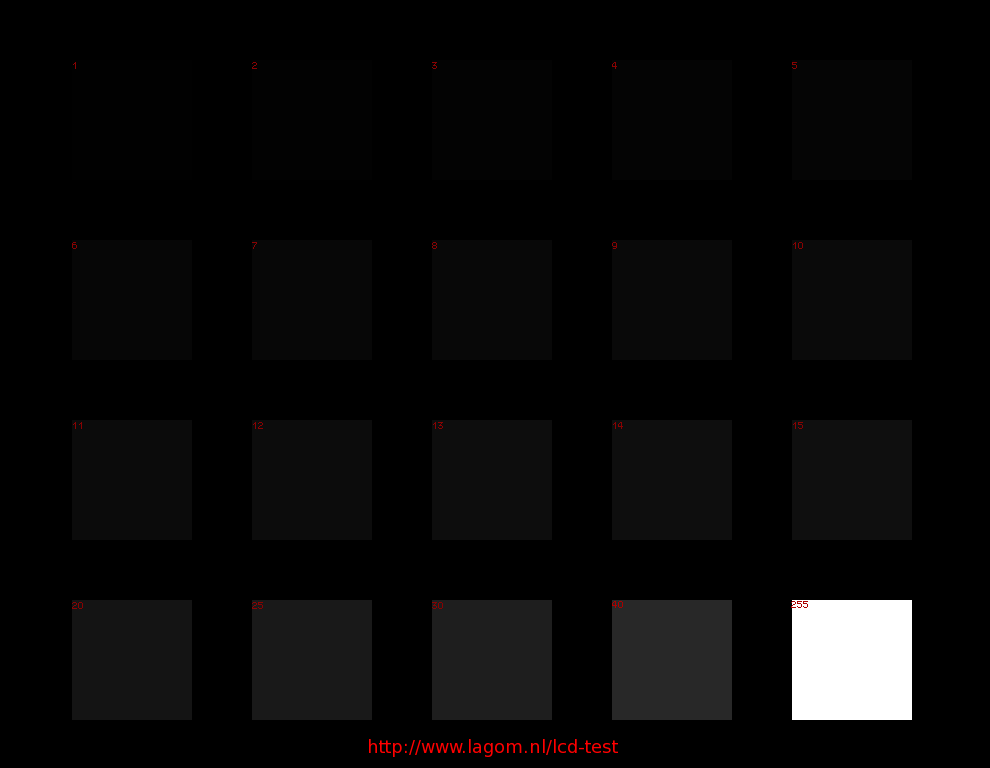
\includegraphics[width=0.35\textwidth]{images/blacktest_example.png}
  \caption[Black Squares Test]{Example of Black Squares Test.\protect\footnotemark{}}
  \label{fig:blacktest_example}
\end{figure}
\footnotetext{"Black Level", Available at: \url{www.lagom.nl/lcd-test/black.php}. Last accessed on September 7th, 2016.}
%
We will present to the user a \textbf{pair of images}, consisting of a set of 10 squares each; in the first of them, we will test the black level of user's monitor, showing each square with a different shade of black, from brighter ones (Square 1) to darker ones (Square 10). The user is, then, asked to express which square is the last, most perceivable, darker square, and point out the word which follows it. The second image has the same job as the first one, except that this rules out the white-level of the monitor and the ten squares present different tones of white. An example of this sort of test is presented in Figure \ref{fig:blacktest_example}. The results of this phase are recorded for further analysis when the study finishes. \par
%
Regarding the laboratory environment, we are going to conduct the user tests in a LCD monitor, under a fixed light source; the monitor will be calibrated
using a colorimeter which will consider the existing light in the environment and adjust the color of each pixel to a standard. The user will be focused on
the task and no other user will be present in the room at the same time, excluding the study regulator; the user will have a fully detailed test protocol to
follow.
%
\textbf{\underline{\emph{(... FALTA TEXTO AQUI ...)}}}
%
Referir limitação descoberta entre Chrome Safari
%
\subsection{Testing Color Vision Deficiencies Phase}
\label{subsec:design_ishihara}
%
\subsection{Core Test Phase}
\label{subsec:design_core}
%
Incluir tabela com todas as cores, igual a folha de auxilio. Referir que Ciano, por erro, não esta a ser testado no formato objTwoColors. \\
Referir aqui que dados estão a ser guardados do utilizador, e como estão a ser guardados, (objTwoColors e twoColorsObj), etc. \\
Referir aqui também que slider contemplava cores standard da folha de calculo para ambiente online,
mas para ambiente laboratorio cores eram antes processadas no Matlab. Slider não tinha cores ordenadas para que utilizador não utilizasse
algum modelo mental e aprendesse previamente a misturar. Cores foram misturadas sem qualque critério (referir ordem pela qual apareciam). \\
Referir aqui caminho do calibrador -> icc -> matlab -> converter cores -> slider \\
Falar de folha de calculo do excel com todas as cores, que depois for migrada para matlab
e convertida de acordo com perfil de calibração. \\
Important detail: color conversion between Excel and adapted colors with ICC profile, Spyder and all. ColorConverter.m. \\
%
\begin{table}[htbp]
  \resizebox{\textwidth}{!} {
  \begin{tabular} {|c|c|c|c|c|c|c|c|c|c|}
    \hline
    User ID & Type & First Color & Second Color & Third Color & Drags & Time & Rating & Resets & Question ID \\ \hline \hline
    5710cca334d60 & objTwoColors & \#0080FF & hsl(58.69565217391305,1,0.50) & hsl(98.15217391304348,1,0.50) & 992 & 117 & 4 & 2 & 10 \\ \hline
    5745c1c07cc0c & objTwoColors & \#8000FF & hsl(300,1,0.50) & hsl(324.13043478260875,1,0.50) & 645 & 55 & 2 & 1 & 14 \\ \hline
    5745350dc1e22 & objTwoColors & \#0080FF & hsl(226.30434782608697,1,0.50) & NONE & 115 & 11 & 5 & 1 & 10 \\ \hline
    57451c3b38192 & objTwoColors & \#00FF80 & NONE & hsl(150,1,0.50) & 462 & 39 & 5 & 1 & 15 \\ \hline
    574511e99b6d9 & objTwoColors & \#0080FF & hsl(15.652173913043478,1,0.50) & hsl(316.30434782608694,1,0.50) & 442 & 40, & 1 & 1 & 10 \\ \hline
    57427cf6bad0c & twoColorsObj & \#00FFFF & \#FFFF00 & \#46FF9C & 6 & 14 & 3 & 1 & 32 \\ \hline
    5740bda9be3dc & objTwoColors & \#FF7200 & hsl(9.130434782608695,1,0.50) & hsl(50.21739130434783,1,0.50) & 45 & 22 & 5 & 1 & 11 \\ \hline
    573c783748e8b & twoColorsObj & \#00FFFF & \#CBFF00 & \#00FF6B & 44 & 25 & 3 & 1 & 32 \\
    \hline
  \end{tabular}}
  \caption[Excerpt of Raw "Results" Table]{Excerpt of Results Table, with raw data.}
  \label{table:csv_resultsraw}
\end{table} \par
%

%
\section{Evaluation Criteria}
\label{sec:impl_evaluationcriteria}
Ishihara plates and more, whatever we consider relevant. Falar também de como a calibração era considerada válida ou não. Erros
que poderiam ser gerados pelo field number html5, que com scrolls podia dar valores errados. \\
